\documentclass[12pt, a4paper,oneside]{report}
\usepackage{titlesec}
\usepackage[utf8]{inputenc}
\usepackage[T1]{fontenc}
\usepackage{textcomp}
\usepackage{framed}
\usepackage{pbox}
\usepackage{caption}
\usepackage[nottoc,numbib]{tocbibind}
\usepackage[pdftex]{graphicx}
\usepackage[toc]{glossaries}
\usepackage{amssymb, amsmath}
\usepackage[colorlinks,
pdfstartview = FitH,
linkcolor = black,
plainpages = false,
hypertexnames = false,
citecolor = black]{hyperref}
\usepackage{setspace}
\setstretch{1.25}
\usepackage[left=3.5cm,right=3.5cm,top=2cm,bottom=2cm]{geometry}
\graphicspath{{./pics/}}
\usepackage[printonlyused]{acronym}
\usepackage{todonotes}
\usepackage{subcaption}
\usepackage{float}
\usepackage{pifont}
\newcommand{\cmark}{\ding{51}}%
\newcommand{\xmark}{\ding{55}}%
\usepackage{multirow}
\usepackage{pdflscape}
\usepackage{eurosym}
\usepackage{tocbibind}
\usepackage[english]{babel}
\usepackage[utf8]{inputenc}
\usepackage{multirow}
\usepackage{subcaption}
\usepackage[section]{placeins}
\usepackage{lscape}
\usepackage{adjustbox}
\usepackage{graphicx}
\usepackage{amsmath}
\usepackage{algorithm}


\begin{document}

\begin{titlepage}
	Universität Passau\newline
	Fakultät für Informatik und Mathematik
	\vspace{2.5cm}
    \begin{center}
    \LARGE\textbf{{Classification  Of Visualization  In Scientific Literature}}\\
   
    \normalsize

    \vspace{2.5cm}
    \end{center}

 \normalsize{
 	Masterarbeit zur Erlangung des akademischen Grades\newline
 	Master of Science (M.Sc.)\newline
 	\ \\
 	Lehrstuhl für Intelligent Systems und Lehrstuhl für Data Science \newline
 	der Fakultät für Informatik und Mathematik\newline
 	der Universität Passau\newline
 	
 
    \begin{tabular}{ll}
    	Name: & Arnold Azeem \\
    	Matrikelnummer: & 79176 \\
    	Fachbereich: & Informatik\\
    	Studiengang: & Master Informatik\\
	Erstprüfer: & Prof. Dr. Christin Siefert \\
	Zweitprüfer: & Prof. Dr. Michael Granitzer\\
	Date: &     \today
    \end{tabular}\\
    }



\newpage
\begin{abstract}
Distinct visualisation techniques are used in scientific research publications to summarise large amount of data and also represent a variety of data. These visualisations help to communicate complex information and support the arguments being presented in the publication in a way that is easy to understand and follow.
These figures tend to reveal trends, patterns or relations that might have otherwise been difficult to grasp using only text. 
It is therefore relevant that we extract the data from these visualisations since the extracted data can be used for validating the publication or presenting the data in another form for a different audience. In this context, classifying these visualisations is the initial step since, there is a variety of visualisations and each one is processed in a specific way. It is only after classification that extraction of raw data from these visualisations can be acquired for other tasks. This thesis presents an approach whereby real world data is used to create four types of plots (scatter plots, bar charts, line charts, and box-plots) and random plots also of the same kind from the Internet are added together and used to train and evaluate a CovNet model to be able to classify these plots. 
\end{abstract}

\renewcommand{\abstractname}{Acknowledgements}

\end{titlepage}
\setcounter{tocdepth}{10}

\clearpage
\tableofcontents


% \begin{acronym}

% \acro{XML} {Extensible Markup Language}s

% \end{acronym}

\listoffigures
\listoftables

\titleformat{\chapter}{\LARGE\bfseries}{\thechapter}{1em}{}

\newpage
\chapter{Introduction}
"A picture is worth a thousand words" even though a widely used phrase stands to be very true especially when complex data is visualized and presented in scientific research publications. 
Data is ever growing and sometimes complex, using figures and diagrams to interpret and represent this data cannot be undermined since, they provide a way to easily give insight into the research findings, which would have otherwise been more complex relying on  only textual data. For this reason, there has been a growing interest in the chart analysis area and quite a number of techniques have been developed. I spite of this growing interest, there has been little groundbreaking results achieved due to different variations in appearance of plots \cite{liu2015chart}.
For example, Manollis Savva, et a \cite{savva2011revision} proposed a model to classify charts using extracted low-level features and textual features. After extracting the features, a  Support Vector Machines (SVMs) classifier is used for the classification step. This method was limited since most charts contain the same type of features like axes, grid lines, and legends.
In V Shiv Naga Prasad's work \cite{prasad2007classifying} classification was based on using features based on the shape and spatial relationships of their primitives. This work was limited due to the inconstancy in which data in most charts can be depicted.
The process of extracting data already visualized as figures can be done relatively easier manually but becomes more complicated if done automatically. This process can be divided into two main steps \cite{savva2011revision}. The first step which our work focuses on, classifying the chart and the second step which involves extracting the data from the classified chart.
To achieve the classification step, this paper presents an approach where charts are created with real-world datasets, different plotting programs (Python, Matlab, R, and Java) and different libraries supported by these plotting programs were used together with downloaded chart images from the Internet. We then use these images as input to Convolutional Neural Network (CNN). CNN was used instead of primitive approaches because it has achieved ground breaking results in the area of image classification \cite{amara2017convolutional}. Our model can identify four classes of plots namely Box-plots, Line Charts, Scatter-plots and, Bar-charts.
The other parts of this paper are organized in the follows: 
In the next Sections, we present the motivation behind this work. Other works related to this,  our proposed method is described,
Experimental evaluation and results are reported, and finally, the conclusion and the way to approach this work in the future.

\section{MOTIVATION}
Complex data is better explained in scientific papers with the aid of visualizations. These plots present complex data in an easy to understand way compared to textual representation. The data which these visualizations contain when extracted play an important role in events where another researcher wants to verify the work of the publisher, this data can also be used to develop other visualizations in situations where the paper needs to be presented to a different audience with a different background as opposed to the audience which the visualizations were created for, Also when comparing two plots the raw data helps make a better decision than just the figures. Since each plot will be processed differently to extract the raw data, it very relevant that we can distinguish one plot from another and this is the main aim of this thesis. 

\section{OBJECTIVE}
The purpose of this thesis is to answer the question: \begin{quote} How Well Can We Classify the Four Different Types of Plots (Line Chart, Bar Chart, Scatter Plot and Boxplot) in Scientific Literature ? \end{quote} In this work we focus on only four plots. These plots are scatter plots,bar charts,line charts and Box plots. Figure \ref{fig:vis} shows the vision of this work, The first part of the diagram involves extracting or obtaining  the four different types of plots mentioned earlier,after which we then label our plots and train a neural network model to be able to classify with high accuracy any of the four plots if shown to our model, then finally the raw data can be extracted from the detected plot.
But this work mainly focuses on the red dotted lines shown below in the diagram which which is getting the plots, labeling them, training the model and classifying the plots. \\

\begin{figure}
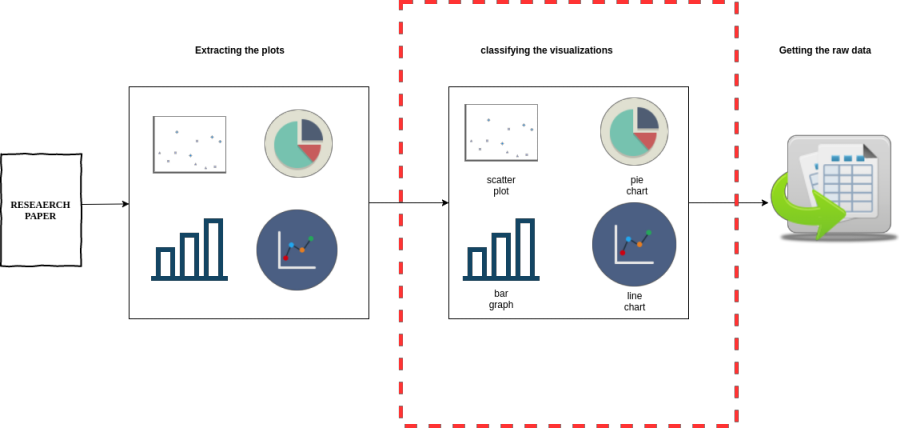
\includegraphics [scale=0.5] {vision}
\captionof{figure}{What we hope to achieve in the thesis}
\label{fig:vis}
\end{figure}

\chapter{Background and Related Work}
Classification involving charts has been a topic of huge interest in recent times. This is due to the fact that most publication are embedded  with these charts as a way to convey complex research findings in more visualizable and easy to understand form. As a result of its popularity different techniques have over time been used for classification of charts and these techniques have evolved over the years. 
The techniques can be put into two categories; Model Based Approaches and Machine Learning Based Approaches ~\cite{amara2017convolutional}. Next the approaches will be explained into details.

\section{Model Based Approaches}
The following is written with inspiration from Boyle et al. work~\cite{boyle2007advances}. Many chart are very different in sense of their context structure. This is as a result of the variability of positions of the context structure of a chart. Content like; legends, axes, grids etc have no fixed positions and sometimes are not even present in some charts, as a result classifying becomes a difficult task. The model based approach is divided into two steps. Firstly, a number of predefined object classes are created with abstract models and then an image is matched with the created model. For example, a model for a 2D/3D pie chart consists of line segments (radii and circular/elliptical arcs), and these line segments are used to create the model, however, just using these line segments wont be enough, so some constraints are introduced into the model, example of constraints of a pie chart include; the center of the pie chart is where all radii meet; all 2D pie charts have radii of equal length; arcs mainly form parts of the same 2D pie chart circle, or if its a 3D then the arcs form part of the ellipse. After this a goodness-of-fit is introduced to help measure the discrepancy between the image and the conditions for the model. For example, a goodness-of-fit of a pie chart is as follows: difference in length of radii; difference in how the arcs are curved; distance between a center of a circle and that of a radii. When a chart is presented for classification, the edges are detected, thinned, linked, vectorized, extracted and compared to the various edge models created and the best match is selected. After this, the good-to-fit criteria is used to measure the difference between the edges of the model and the image. Finally, a voting is performed base on the value of the good-to-fit results. The model based approach has some draw backs though. The main drawback is that human intervention is needed to develop the various models. This could be a cumbersome and time consuming procedure. Due to the limitation of this approach a machine learning approach was introduced to handle some of the model based approach drawbacks.


\section{Machine Learning Based Approaches}
This approach also has different method. Some methods 
involve using handcrafted features from the charts for classifying the chart. In Zhou and Tan's ~\cite{zhou2000bar} work, features like legend, x-y-axis title, chart title and value of the bar were extracted for purposes of classifying a bar-chart. In Shao and  Futrelle's~\cite{shao2005recognition} work, graphical elements of the charts like colors,tick marks on an axis and data point markers are used. Another instance where handcrafted features were used was in Inokuchi et al. work~\cite{inokuchi2000apriori}. In this work regularly appearing substructures of chart are extracted and used as features for classification. The next step is the classification step, after the features are obtained, they are then represented in vector form for the classification stage. The features are stored in a matrix vector like structure. Algorithm~\ref{alg:1} shows an example structure. This structure has columns containing the features and one column indicating the target or label of the chart. The structure is then fed as input into a machine learning technique for the model training step. In Karthikeyani and Nagarajan's paper~\cite{karthikeyani2012machine} after the features were obtained SVM Classification \footnote{http://www.statsoft.com/Textbook/Support-Vector-Machines} MLP Classification
\footnote{http://www.iro.umontreal.ca/~bengioy/ift6266/H12/html/mlp\_en.html} and  KNN Classification\footnote{
https://kevinzakka.github.io/2016/07/13/k-nearest-neighbor/} were used to create a function that maps the set of features to a predefined label. This function is known as the classification model. This technique also achieves very good results but, the drawback is the reliance on handcrafted features such as edges and corners and therefore, does not handle a large amount of data with variable context properly. Recently however, CovNets (this abbreviation stands for Convolutional Neural Networks and will be used a lot through this work) \footnote{https://deeplearning4j.org/convolutionalnetwork}, a machine learning technique which does not need to be supplied with handcrafted features, since they learn the features and classify them on their own. Hence, CovNets are used in our work to automatically classify charts and avoid the cumbersome task of having to extract handcrafted features.


\subsection{Convolutional Neural Network}
The following is inspired by the following blogs by ujjwalkarn \cite{cnnonline}, Ifu Aniemeka\cite{AFriendl79} and Adit Deshpande \cite{convo:online}.
CovNets are a variety of Artificial Neural Network which have given results near to human performance. They  especially perform well in the areas of image recognition and classification. All CovNets are divided into steps called layers, the layers are Convolution, Pooling or Sub Sampling, Classification (Fully Connected Layer). When an image is presented to a computer, the image is seen as an array of pixel values. For instance if a  color image of size 48x48 is presented the computer sees it as 48x48x3 where the 3 represents the RGB values. 

\subsubsection{Convolutional Layer}
The convolutional layer will be explained using the following example, let consider the image as a magical cake of height and width 48x48, and there is a cake cutter of size say 5x5. The cutter is used to cut the cake from the top left. The cutter is referred to as a filter in machine learning. The cutter in this case is also an array of numbers called weights and for the maths to work the cutter must have the same depth as our cake (5x5x3).
Lets first consider the cutter being in the first position ie. the top left of the cake. The values in the cutter are multiplied with the values of the cake (element wise multiplications). These multiplications are all summed up and result in a single number. This single number is only for the first part and this process is repeated through out the whole cake (Next step would be moving the cutter to the right by 1 unit, then right again by 1, and so on) keep in mind its a magical cake so you can cut a part more than once. After using the cutter on the whole of the magical cake we result in a new cake of size 28x28x1, the results is called a feature map. The filters are low level feature identifiers (straight edges, simple colors, and curves). 


\subsubsection{ReLU Layer}
The next layer after the convolution phase is the Rectified Linear Units (ReLU). This layers helps to handle situations where the relation between the input values and the CovNet output is non-linear. The ReLU has a function \(f(x) = max(0,x)\) which means if you give it a value x, it will return 0 if x is negative and will return the value itself if its positive. There are also other functions which can used n place of the ReLU; that is the tanh or the sigmoid function but the ReLU mostly works well.

\subsubsection{Pooling Layer}
The pooling layers basically have two main functions, first one is that it helps the CovNet to locate features regardless of which part of the image it is located. This results in the model being robust against small changes in position of the features of the images. The second function is that it also helps to reduce the size of the feature map. Therefore computations in the futures layers are relatively less complex. One way of performing pooling is using max pooling technique, thats is sliding a window through the feature map, the windows fills a number of arrays in the feature map therefore, you pick the largest among all the numbers and disregard the rest of the numbers. 

\subsubsection{Fully Connected Layer}
This is the last layer and where the decision about the image is made. i.e a probability saying which class the image belongs to. This layer takes the output of the previous layers, which are the high level features and check which class these features strongly correlate to. All the above mentioned layers can be multiply stacked 
on each other.
In the rest of this chapter, three related works that our work builds on are described into details.  

\subsubsection{Machine Learning Classification Algorithms to Recognize Chart Types in Portable Document Format(PDF) Files}
Karthikeyani and Nagarajan's work ~\cite{karthikeyani2012machine} focuses on classifying charts found in pdf files. Th steps involve extracting texture features from the charts and then, using a machine learning technique for the classifying phase.
The dataset consists of images extracted from various pdf's. The dataset consists of 155 images in total and  images are 256*256 RGB. Table~\ref{table:pdf} shows the details of the dataset used. In this work, handcrafted features are extracted from the image and then used in the classification phase to train and test a model.
For the feature extraction phase, Gray Level Co-Occurrence Matrix (GLCM) is employed. GLCM is a technique which uses co-occurrence matrix to extract texture features of an image with the use of statistical equations. GLCM was used to extract eleven features, these included: area, median, minimum and maximum intensity, contrast, homogeneity, energy, entropy, mean, variance, standard deviation and correlation. These extracted features are correlated to the pixels of the image. These extracted features are then stored using a 2-dimensional matrix vector data structure. This structure has thirteen (13) columns and 'x' rows, where x is the size of the dataset. The features are stored in twelve (12) columns and the label is stored in the thirteenth column. The features and labels were stored in the below structure~\ref{alg:1}.

\begin{table}[h]
	\centering \def\arraystretch{1.5} \small
	\begin{tabular}{|p{3cm}|p{3cm}|p{3cm}|p{3cm}|}
		\hline
		Chart Type & No of Charts & Chart
		Type & No of Charts  \\ \hline
		2D Bar chart & 40 & Doughnut 2D & 7 \\ \hline
		3D Bar chart & 16 & Doughnut 3D & 11\\ \hline
		2D Pie chart & 13 & Line & 35 \\ \hline
		3D Pie Chart & 20 & Mixed Chart& 13 \\ \hline
	\end{tabular}
	\caption {Details on Dataset from \cite{karthikeyani2012machine} }	
	\label{table:pdf}
\end{table}


\begin{algorithm}
\caption{This is the structure used to store the features}
\label{alg:1}
Struct FeatureVector \{\\
	float feature1; float feature2;\\
	float feature3; float feature4;\\
	float feature5; float feature6;\\
	float feature7; float feature8;\\
	float feature9; float feature10;\\
	float feature11; float feature12;\\
	int target;\\
\}
\end{algorithm}


This vector like structure is then fed as input into three classifiers SVM, MLP neural network and K-Nearest Neighbour. These classifiers are then trained and a classification model is formed for the recognition step. After this, to see if the model works well a test set consisting of new records is fed into the model for the model to predict their labels. Three metrics were used to check the performance of the model; error rate,
classification accuracy and speed of classification. The error rates are MLP 0.30, K-NN 0.22 and SVM 0.23. For the accuracy metric; KNN (78.06\%), MLP (69.68\%) and SVM (76.77\%). Finally the speed metric, which sum of training and test time results in MPL being the slowest with 8.38,followed by SVM with 0.31secs and  KNN with 0.26secs. Even though these results were very good the paper proposed, extracting features which are relate to shape and curves.

\subsubsection{Architecture proposal for data extraction of chart images using Convolutional Neural Network}
Our work is inspired by De Freitas et al.~\cite{junior2017archi}, proposed a way to extract the wealth of information contained in different visualization techniques. The paper talks about two main stages of accomplishing this task. Firstly, classification of the charts is done since it allows a different variety of chart to be detected automatically allowing the next step, which is the extraction of data from the classified plots. The paper, however, focuses on the first step, classification of charts. In this paper, a Convolutional Neural Network is used for the classification task. The Convolutional neural network encapsulates the characterization and classification processes during its learning process, unlike other techniques. The dataset used for this task were searched for and downloaded from Google image search. Table \ref{table:rela} shows the chart types which were collected and the number of train and test sets which the respective charts were divided into.

\begin{table}[h]
	\centering \def\arraystretch{1.5} \small
	\begin{tabular}{|p{5cm}|p{3cm}|p{3cm}|}
		
		\hline
		Chart Type & Test & Train \\ \hline
		Area Chart & 50 & 555 \\ \hline
		Bar Chart & 50 & 657 \\ \hline
		Line Chart & 50 & 489 \\ \hline
		Map & 50 & 476 \\ \hline
		Pareto Chart & 50 & 261 \\ \hline	
		Pie Chart & 50 & 361 \\ \hline
		Radar Chart & 50 & 454 \\ \hline
		Scatter Chart & 50 & 552 \\ \hline
		Table & 44 & 236 \\ \hline
		Venn Diagram & 48 & 304 \\ \hline
		Total & 498 & 4345 \\ \hline
		
	\end{tabular}
	\caption {Number of Train and Test Dataset collected}	
	\label{table:rela}
	
\end{table}
For the classification, a variant of CovNet called LeNet-based CNN model is used. The model was implemented using Tensorflow\footnote{https://www.tensorflow.org/}, LeNet-based CovNet has an architecture which is comprised of 3 convolutional layers, followed by a fully connected layer. The model is trained in a way that the dataset is divided into mini-batches, samples of fixed sizes(100) are selected and fed into the CNN, as a result of this process the model becomes robust since it learns to generalize from the different min-batches which are fed into the model. Also, all the images are converted to JPG and resized to 224x224x3, that is, 224 pixels of height, 224 of width and 3 layers of output. The other parameters used were 1000 epochs and a learning rate of 0.003. The accuracy at the end of the training process was 70\%.

\subsubsection{Chart classification by combining deep convolutional networks and deep belief networks}
In another paper by Liu et al.~\cite{liu2015chart}, a new approach was proposed for the process of chart classification. The process involves using CovNet to extract deep hidden features of charts and then deep belief networks then use the extracted features to predict the labels of the charts. Due to a difficulty in acquiring a large number of charts as training data, natural images where first used to train the model and later the model was fined tuned with just over 5,000 collected charts. The types of charts collected were pie charts, scatter charts, line charts, bar charts, and flowcharts. The architecture of the CovNet is made up of five Convolutional layers and two fully-connected layers and then an output layer. The preprocessing steps for the images involve down-sampling them to 256 x 256 x 3, after which each is cropped to a size 227 x 227 from the center and its horizontal flip are extracted as the input of the CovNet, other parameters used for the CovNet include a learning rate that starts with 0.01 initially and is then decreased by a factor of 0.1 after every lOOk iterations, the weight decay parameter was set at 0.0005 and a dropout rate of 0.5. This results in an output of a 5-way softmax which produces the distribution over the 5 class labels and this is used as input for the deep belief network. The deep belief network architecture has three hidden layers, whose dimensions are 5000, 500 and 2000. This results in a softmax predicting the probability
distribution over the 5 categories of charts as output.
The training process was done with 4000 randomly selected images and the rest were used as test set. The accuracy of the model after the evaluation was  75.4\%. Table \ref{table:deep} show the results after the training was done without deep belief networks but pre-trained with the natural images and finally the training done with only the chart dataset but with deep belief networks.

\begin{table}[h]
	\centering \def\arraystretch{1.5} \small
	\begin{tabular}{|p{3cm}|p{3cm}|p{3cm}|p{3cm}|}
		
		\hline
		Chart & CovNets&CovNets+DBN without pre-training & CovNets+DBN \\ \hline
				
		Bar Chart & 75.6\% & 45.6\% & 74.2\% \\ \hline
		Flow Chart & 88.3\%  & 56.8\% & 91.3\%  \\ \hline
		Line Chart  & 71.2\%  & 22.3\% & 67.9\% \\ \hline
	
		Scatter Chart & 69.8\% & 44.5\% & 84.2\% \\ \hline
		Pie Chart & 58.1\%  & 50.1\% & 59.4\%    \\ \hline
		Ave. Accuracy & 72.6\%  & 43.9\% & 75.4\% \\ \hline
		
	\end{tabular}
	\caption {Comparing Results of Proposed Framework from (Liu et al.~\cite{liu2015chart}) }	
	\label{table:deep}
	
\end{table}


\chapter{Approach}
As seen in the previous chapter, different approaches and methods have been described for chart image recognition. Due to the complexity of this task, a CovNet approach is employed for our work. Reasons for selecting this approach include; automatic capturing, learning and extraction of features; parameter sharing which allows the model to learn a single set of weights once, rather than a different set of weights every time~\cite{Rodriguez} and more importantly a performance accuracy nearing human capability. In spite of all the advantages of CovNets, they are very computationally expensive to apply on high resolution images. Fortunately, current GPU capabilities with the help of good optimization techniques can handle this issue~\cite{krizhevsky2012imagenet}. \newline\newline
The specific contributions of this work is as follows: to create a dataset of chart images (scatter-plot,bar chart,line-chart and box-plot) using real world data. This chart image dataset tries to capture all variety of structure in the various chart images to be handled. The scripts, libraries and parameters used in creating the  chart images will readily available for recreation of the dataset. The second contribution, is training a CovNet model for recognizing these types of chart images when presented to it.\newline
The rest of this chapter describes into details how the dataset was created, it also describes the CovNet architecture that was used for the classification task.

\section{Dataset}
The following paragraph is inspired by \cite{edi}.
The saying 'Garbage in Garbage out' is a valid statement when it comes to creating a dataset for machine learning. The machine learning technique will learn from whatever data fed to it. So if a dataset of good quality is fed into the algorithm, then the model created will also be of good quality. The dataset creation stage is therefore a very important stage. In most approaches that worked on chart images classification, the dataset used consisted of images downloaded from Google and a few others were obtained from extracting them from pdf's. This approach we believe is bit limited since, we don't know the programming languages, the libraries used and parameters used in creating these charts. This information is very relevant since it tells us how diverse our resultant dataset is. For example, how are we sure that all the charts that were downloaded from Google, were not only created with python or java?, and in such case how well will a new chart created with matlab or R be classified. For this reason the dataset comprised of image charts created with different libraries and in different programming languages. In the next sections, the various datasets and the languages used in plotting are described. To make the dataset as diverse as possible, charts created in each programing language used a different set of CSV files. 

\subsection{Dataset for Matlab}
The Data used for creating the plots in Matlab were randomly chosen from Project Dataset \cite{projectdataset}, a free CSV data repository, DatPlot \cite{datplot} and Plotly CSV repository in github \cite{plotly}. The datasets are multidimensional and compiled from normal day to day activities like dating, what makes people happy etc, and objects like cameras and cars. On the average the datasets used contain about 500 instance and 5 different columns. The biggest dataset is called Speed dating data. It is made up of over 8,000 observations of answers to survey questions about how people rate themselves and how they rate others on several dimensions. The smallest dataset used has 33 instances and 12 columns. It contains information about cars. The number of gears and speed, just to name a few attributes.

\subsection{Dataset for R}
For the plots in R, 13 random CSV files where downloaded from an archive of datasets distributed with R called Rdatasets  \cite{rdata}. Rdatasets is a collection of dataset distributed with R. On the average there are 80 instances and 5 columns in each dataset.
The biggest CSV file is the Australian athletes dataset. It's made of 203 instances and 14 columns and contains attributes like sex,height,weight and sports. The smallest dataset is the Canadian Women's Labour-Force Participation. This dataset has 30 rows and 7 columns. It contains information like average wages of women, percent of adult women in the workforce etc.


\subsection{Dataset for Python}
The data used for creating the plots in Python were 15 randomly seleted csv files also from  Rdatasets \cite{rdata}. The biggest dataset among the 15 is the Monoclonal gammapothy data, it contains natural history patients with monoclonal gammapothy of undetermined significance. The dataset is made up of 1384 observations with 10 columns, it has attributes like age, sex, time of death and last contact in months. On the average each dataset contains about 200 instances and 7 columns of multi-dimensional data. The smallest dataset however contains only 33 instances with 11 columns and is called the Nuclear Power Station Construction Data.The data relate to the construction of 32 light water reactor (LWR) plants constructed in the U.S.A in the late 1960's and early 1970's.

\subsection{Dataset for Java}
For the plots created in java, I used the dataset made available by Plotly \cite{plotly}, a github repository of CSV datasets used in the Plotly API examples. 14 random CSV files were downloaded, the biggest file has 1002 instances and 9 columns, and on the average each file contains about 100 instances and 9 columns. The smallest file however is made of 33 instances and 12 columns called the mtcars file. It contain information about a variety of different car models like the number of gears, speed etc. The table \ref{table:1} contains the names of all CSV files that were used in the different languages with the different plotting programs.



\begin{table}[h]
	\centering \def\arraystretch{1.5} \small
	\begin{tabular}{|p{5cm}|p{3cm}|p{3cm}|p{4cm}|}
		
		 \hline
		 \multicolumn{4}{|c|}{Datasets} \\
		 \hline
				
		Python & Matlab & R  & Java\\ \hline
		
		3d\_line\_sample\_data.csv \par LightFordwardFlapStall.csv  \par line\_3d\_dataset.csv \par
		longley.csv  \par loti.csv  \par lung.csv  \par nuclear.csv  \par timeseries.csv  \par
		USJudgeRatings	\par WVSCulturalMap.csv  \par wind\_rose.csv  \par volcano.csv  \par uspop2.csvm \par tips &
		
		Camera.csv \par Cars.csv \par speedDating.csv \par Cereal.csv  \par happiness.csv \par TestData1.csv \par TestData2.csv  \par mpg.csv \par okcupid-religion.csv  \par spectral.csv
		\par stockdata.csv \par subplots.csv  & 
		
		ais.csv \par Angell.csv  \par Baumann.csv \par Bfox.csv \par cane.csv \par carprice.csv \par Chirot.csv
		Davis.csv \par Ericksen.csv \par Florida.csv \par Highway1.csv \par Pottery.csv \par Prestige.csv 
		salinity.csv \par urine.csv & 
		
		3d-line-plot.csv \par 3d-scatter.csv \par 2011\_flight\_paths.csv \par 2011\_us\_exports.csv \par auto-mpg.csv \par candlestick\_dataset.csv \par finance-charts-apple.csv \par 
		globe\_contours.csv\par hobbs-pearson-trials.csv \par motor\_trend\_tests.csv \par 
		nz\_weather.csv \par volcano.csv \par iris.csv \par mtcars.csv	\\ \hline
		
	\end{tabular}
	\caption {Names of datasets used in each plotting program}	
	\label{table:1}
\end{table}


\section{Creating Plots}
The inspiration for creating a variety of plots to capture all type of plots used in scientific papers was gotten by inspecting the dataset of Architecture proposal for data extraction of chart images using CovNet paper \cite{junior2017archi} and Viziometrics: Analyzing visual information in the scientific literature \cite{lee2018viziometrics} dataset. Scripts in various languages were written to handle the plotting and labeling process automatically. All datasets for a particular plot (example scatter plot for python) are put into one folder. The scripts reads each CSV file column by column while creating the plots.
 
Table \ref{table:2} describe how the plots where created in each language. The type column describes the different variety of a particular plot, for example bar charts can be of type stacked, grouped, vertical and horizontal bar charts, also scatter plots types can be a scatter plot consisting of one type of marker, one scatter plot with multiple markers and finally a scatter plot with a line showing the correlation between the plots. 
Figure \ref{fig:fig11} shows two different types of bar charts. Figure \ref{fig:fig1} is a stacked bar chart and  Figure \ref{fig:fig2} a normal vertical bar chart.
The Library column shows the different plotting libraries used, the parameter column describes parameters that were changed and finally the number of plots created were also added. The images below the tables are sample images that exist in our dataset of created plots for each language.

	
\begin{table}[]
	\centering \def\arraystretch{1.5} \small
	\caption {Overview of the varied parameters for creating plots in the different plotting programs}
	
	\label{table:2}
	\begin{adjustbox}{width=\textwidth}
	\begin{tabular}{|p{3cm}|p{3cm}|p{3cm}|p{2cm}|p{4cm}|}
		\hline
		\multicolumn{5}{|c|}{SCATTER PLOTS} \\
		\hline
		
	Language & Library & Parameters & Number of plots  & Type\\ \hline
		
	Python & Matplotlib v2.1.2 \par Plotly v2.5.1 \par Seaborn v0.8.1 & MarkerStyle \par 
	['o', '*', '.', '+','x'] & 1020 &  \multirow{6}{*} {\shortstack { Unique markers, \\ With legends,\\ multiple markers \\ regplot }} \\ \cline{0-3}	   
		  
	MATLAB & Default \par Plotly &  MarkerStyle \par ['o', '*','+','x','s'] & 1044  &   \\ \cline{0-3}	   
		
	R  & Plotly \par Lattice \par Ggplot2 &  MarkerStyle \par ['o', '*', '+','x','s'] & 1644  &  \\ \cline{0-3}		
	
	JAVA & XChart 3.5.1\par jfreechart 1.0.1 & MarkerSize (15 -18) & 1644 &  \\ \hline
	

		\multicolumn{5}{|c|}{BAR CHARTS} \\
		\hline
		
		Language & Library & Parameters &  Number of plots & Types(bar)  \\ \hline
		
		Python & Matplotlib v2.1.2 \par Plotly v2.5.1 \par Seaborn v0.8.1 &   &  1000 &  \multirow{6}{*} {\shortstack {Horizontal and Vertical, \\ Stacked, \\ Grouped bar charts }} \\ \cline{0-3}	 
		
		MATLAB & Default &  Width of bar(14-16) & 1000  &  \\ \cline{0-3}
		
		R & Default,Plotly \par R Library \par ggplot2 & space (0-3)  & 1144  & \\ \cline{0-3}
		
		JAVA  & XChart 3.5.1 \par jfreechart:1.0.192 \par javafx.scene & PlotOrientation \par (vertical or horizontal) \par with error bars & 1144 & \\ \hline
		
			\multicolumn{5}{|c|}{LINE CHARTS} \\
			\hline
			
			Language & Library & Parameters &  Number of plots & Types(Line with)  \\ \hline
			
			Python & Matplotlib v2.1.2 \par Plotly v2.5.1 \par Seaborn v0.8.1 & Linestyle \par ['-', '--', '-.', ':']   &  1000 &  \multirow{6}{*} {\shortstack { Markers, \\ Multiple Lines }} \\ \cline{0-3}	 
			
			MATLAB  & Default\par Plotly &  MarkerStyle \par ['o', '*', '.', '+','x','s'] \par markersize [8-10] & 1000 &  \\ \cline{0-3}
			
			R & Default,Plotly \par R Library \par ggplot2 &  & 1644  & \\ \cline{0-3}
			
			JAVA & XChart 3.5.1 \par javafx \par JFreeChart & MarkerSize (12-16) & 1644 & \\ \hline
			
				\multicolumn{5}{|c|}{Box Plots} \\
				\hline			
				Language & Library & Parameters &  Number of plots & Types(Box with)  \\ \hline
				
				Python  & Matplotlib v2.1.2 \par Plotly v2.5.1 \par Seaborn v0.8.1 &   &  1000 &  \multirow{6}{*} {\shortstack { Notches, \\ Multiple Boxes }} \\ \cline{0-3}	 
				
				MATLAB   & Default &   & 1000  &  \\ \cline{0-3}
				
				R & Default,Plotly \par R Library \par ggplot2 &  & 1644  & \\ \cline{0-3}
				
				JAVA   & XChart 3.5.1 \par Jfree & LegendPosition (topleft,topright) & 1644 & \\ \hline
				
	\end{tabular}
		
\end{adjustbox}

\end{table}


\begin{figure}[!htbp]
	\begin{subfigure}{.5\textwidth}
		\centering
		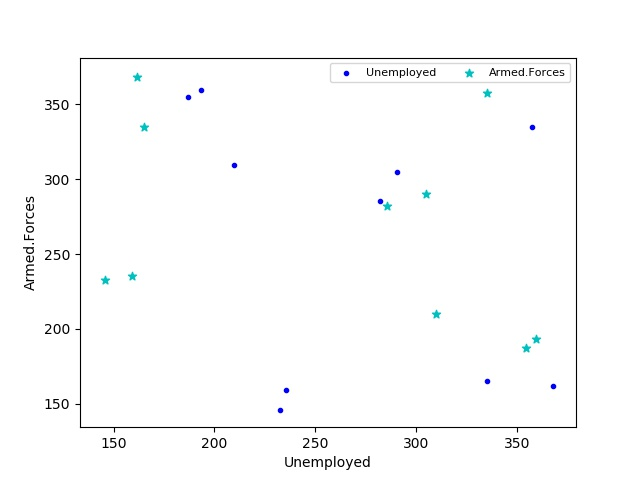
\includegraphics[width=.8\linewidth]{scatter1}
		\caption{Matplotlib scatter plot with star and circular markers }
		\label{fig:fig1}
	\end{subfigure}%
	\begin{subfigure}{.5\textwidth}
		\centering
		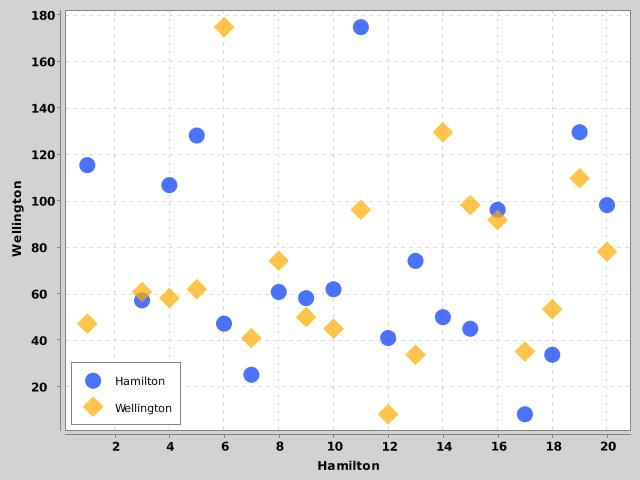
\includegraphics[width=.8\linewidth]{scatter2}
		\caption{Java scatter plot with circular and diamond markers}
		\label{fig:fig2}
	\end{subfigure}
	\caption{Scatter plots}
	\label{fig:fig11}
\end{figure}


\begin{figure}[!htbp]
	\begin{subfigure}{.5\textwidth}
		\centering
		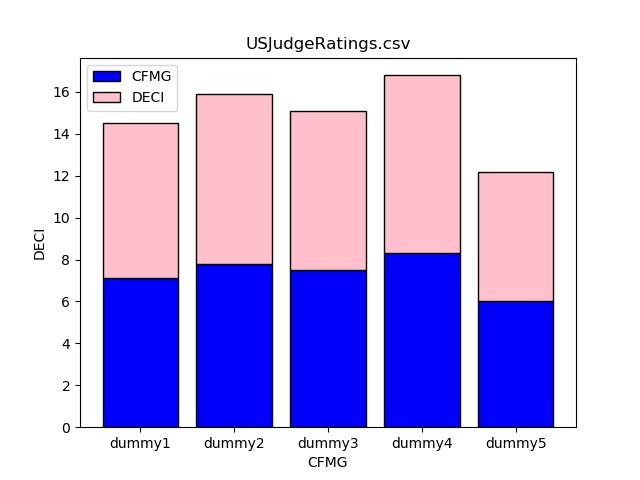
\includegraphics[width=.8\linewidth]{bar1}
		\caption{Matlab stacked bar chart (bar width 16) }
		\label{fig:sfig1}
	\end{subfigure}%
	\begin{subfigure}{.5\textwidth}
		\centering
		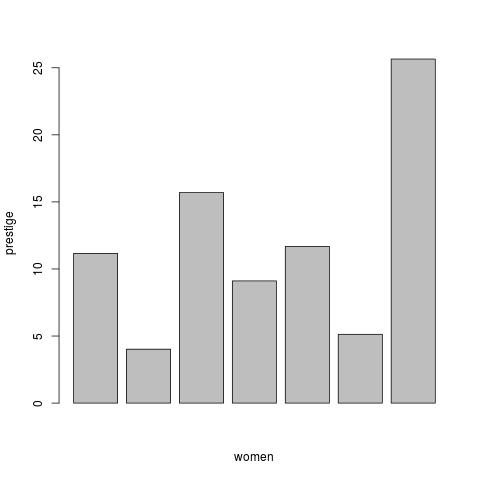
\includegraphics[width=.8\linewidth]{bar2}
		\caption{R horizontal bar chart (bar width 16)}
		\label{fig:sfig2}
	\end{subfigure}
	\caption{Example Bar Charts}
	\label{fig:fig}
\end{figure}


\begin{figure}[!htbp]
	\begin{subfigure}{.5\textwidth}
		\centering
		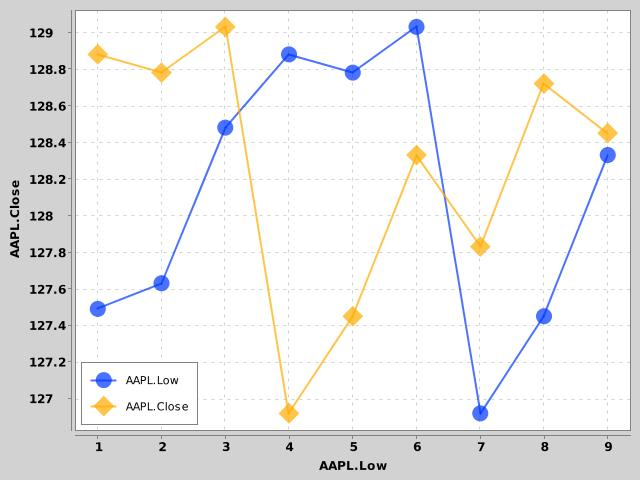
\includegraphics[width=.8\linewidth]{line1}
		\caption{Java line chart with diamond and circular markers }
		\label{fig:sfig1}
	\end{subfigure}%
	\begin{subfigure}{.5\textwidth}
		\centering
		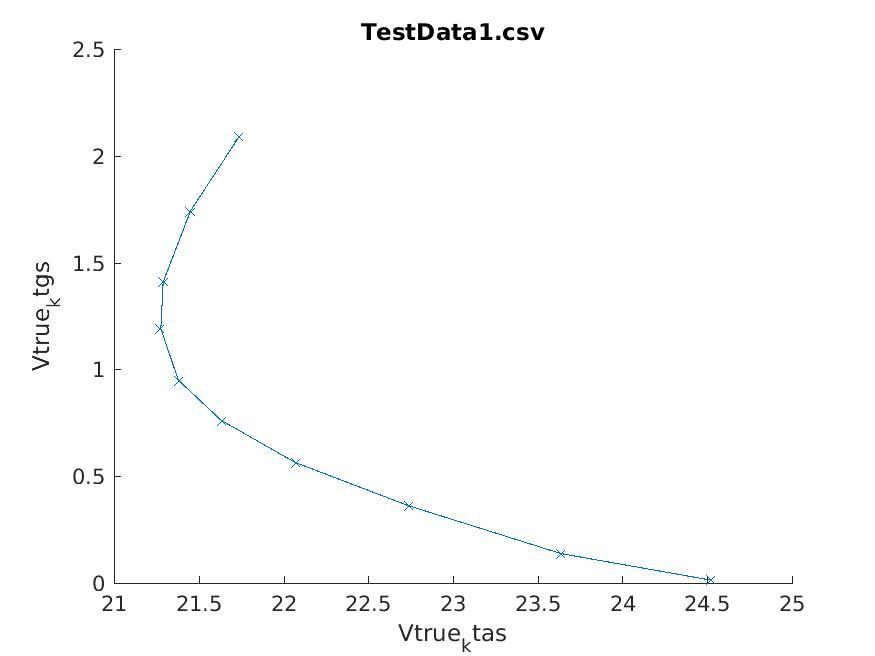
\includegraphics[width=.8\linewidth]{line2}
		\caption{simple Matlab line chart with Asterix marker}
		\label{fig:sfig2}
	\end{subfigure}
	\caption{Example Line Charts}
	\label{fig:fig}
\end{figure}



\begin{figure}
	\begin{subfigure}{.5\textwidth}
		\centering
		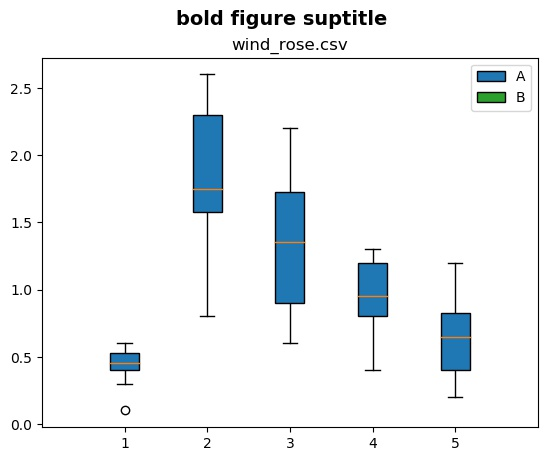
\includegraphics[width=.8\linewidth]{box1}
		\caption{Vertical multiple boxplots in python}
		\label{fig:sfig3}
	\end{subfigure}%
	\begin{subfigure}{.5\textwidth}
		\centering
		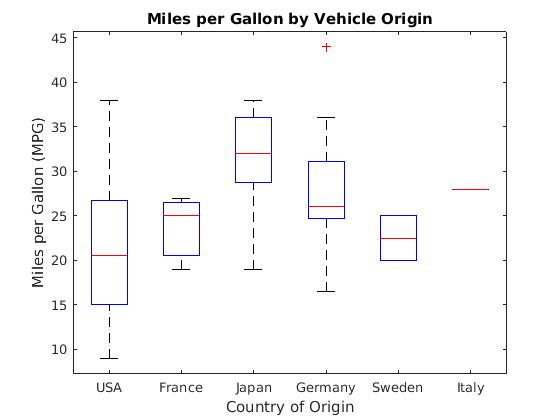
\includegraphics[width=.8\linewidth]{box2}
		\caption{Vertical multiple boxplots in Matlab}
		\label{fig:sfig3}
	\end{subfigure}
	\caption{Example Box Plots}
	\label{fig:figbox}
\end{figure}


\section{Training, Validation and Test set}
Figure ~\ref{fig:approach} summaries how our dataset was split for various activities. In machine learning, a model is an artifact created during the training phase, this model can be likened to a function that maps specific features to their respective labels, the model is trained with a portion of the dataset called the train set. As the model is trained, the validation set is used to decide and pick which metric out of hyper-parameters, early stopping and architecture considerations yields the best performance. These help to adjust and optimize the model~\cite{validation}.Finally, the test-set in machine learning, is the other portion of the dataset which was not used during the training phase. The test-set checks how well the trained model performs on unseen data by giving an unbiased assessment of the model. For this work, the dataset is divided into train, validation and test set. The validation set is not shown in the figure since it forms part of the train data.
\begin{figure}
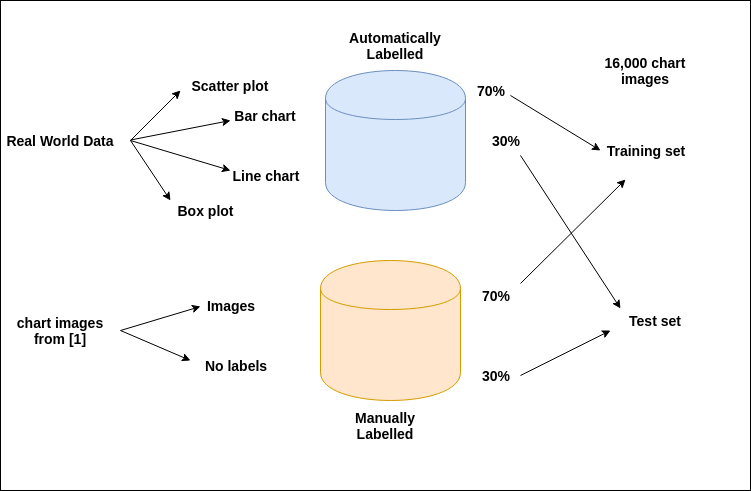
\includegraphics [scale=0.5] {approach}
\label{fig:approach}
\captionof{figure}{Steps involved in building the Classification model}
\end{figure}


\section{The Architecture}


\section{Image Preprocesing}
Image preprocessing is a very important step in any image based application. This process involves taking the image and improving it in a way that enables easier machine understanding. This ultimately makes it easier for the machine to extract important features for other operations. 

\chapter{Evaluation}


\chapter{Summary}

\bibliographystyle{unsrt}
\bibliography{sample}

\end{document}=====